\newpage

\section{Purchase Instrumentation Equipment}

In this class you’re going to build some circuits that will enhance
your learning experience. Rather than just solving problems by hand
you’re going to take and analyze data. Over the summer of 2020, I
wrote a textbook with
\href{https://www.tangiblesthatteach.com/shop}{Tangibles that Teach}
and they have graciously 
bundled all components together. The price is \$50 plus shipping so
it’s about the same price as below but you’ll probably save on
shipping from multiple vendors and everything is all in one place
which is nice. There is an
\href{https://www.tangiblesthatteach.com/downloads}{accompanying textbook that can be downloaded} as well. 

When you get your kit familiarize yourself with all of the
components. I created an
\href{https://youtu.be/6sNNQrhnzLE}{unboxing video on Youtube} for you
to take a look. Below is also a photo of all the components.
\begin{figure}[H]
  \begin{center}
    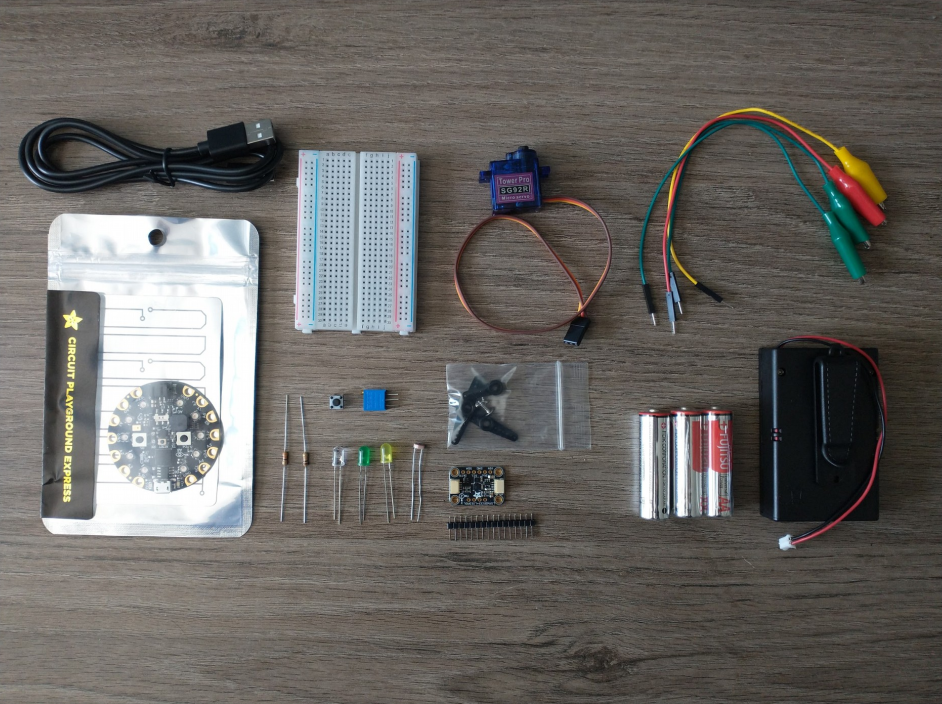
\includegraphics[width=\textwidth]{Figures/components.png}
  \end{center}
\end{figure}

\subsection{Quick Links}

\begin{enumerate}[itemsep=-5pt]
  \item \href{https://www.tangiblesthatteach.com/product-page/instrumentation-kit-for-me-316}{Kit}
  \item \href{https://a2279211-28c1-4f46-9477-0d3265900c7f.filesusr.com/ugd/2413aa_ca39175b0a514b838ec96893b90590eb.pdf}{Document}
  \item \href{https://youtu.be/6sNNQrhnzLE}{Unboxing Video}
\end{enumerate}

\subsection{Turning in this assignment}

\begin{enumerate}[itemsep=-5pt]
  \item Upload a receipt of ALL of your purchases - 50\%
  \item Put your name and the names of your group members. If working
    alone, tell me you are planning on working alone in the PDF you
    upload. In times of COVID, everyone is working alone - 50\%
\end{enumerate}

\newpage

\begin{center}\LARGE{ONLY READ BELOW IF YOU DON’T WANT TO BUY THE KIT
    ABOVE}\end{center}

\subsection{Purchase Items Yourself}

The bill of materials listed below is designed for 2 or 4 students to work together and share
pieces. This kit is not optimized for 3 students. If you are a remote/online student or you just
prefer to work alone then you have the option of purchasing everything yourself. The cost per
student in a group of 4 and 2 is listed as well as the cost if working alone. You’ll find that even
with the optional equipment, the cost of working alone is still less than the price of a standard
college textbook. Note that if you are working alone, be sure to only purchase 1 of each item. If
working in pairs you also have the option of purchasing one of each item. Finally, if you own
some of these components you may wish to simply purchase each item separately. A detailed
parts breakdown is shown after the rubric.

\subsection{Bill of Materials (per 4 students)}

\begin{figure}[H]
  \begin{center}
    \begin{tabular}{|l|c|c|}
      \hline
      Item (ONLY IF YOU DON’T WANT THE KIT ABOVE) & Quantity & Total
      Cost \\
      \hline
      \href{https://www.adafruit.com/product/3333}{Circuit Playground Express (CPX)} & 2 & \$50 \\
      \hline
      \href{https://www.adafruit.com/product/169}{Servo} & 2 & \$10 \\
      \hline
      \href{https://www.adafruit.com/product/592}{USB Cable} & 2 & \$6 \\
      \hline
      \href{https://www.amazon.com/Smraza-Breadboard-Resistors-Mega2560-Raspberry/dp/B01HRR7EBG/ref=sr_1_3?dchild=1&keywords=photocell+circuit+kit&qid=1590531716&sr=8-3}{Electronics Kit} (Photocells, Resistors, Trimpot) & 1 & \$13 \\
      \hline
      \href{https://www.amazon.com/WGGE-WG-026-Pieces-Colors-Alligator/dp/B06XX25HFX/ref=sr_1_1_sspa?dchild=1&keywords=alligator+clips&qid=1613147431&sr=8-1-spons&psc=1&spLa=ZW5jcnlwdGVkUXVhbGlmaWVyPUFLRjlYRVM3SDIySVAmZW5jcnlwdGVkSWQ9QTAwNDczMzEyODNCVTJWSjlMR0NEJmVuY3J5cHRlZEFkSWQ9QTAwMDQyMjkzSlJLNjJRWk9CSVZEJndpZGdldE5hbWU9c3BfYXRmJmFjdGlvbj1jbGlja1JlZGlyZWN0JmRvTm90TG9nQ2xpY2s9dHJ1ZQ==}{Alligator Clips} & 1 & \$4 \\
      \hline
      {\bf Total} & & {\bf \$83} \\
      \hline
      {\bf Cost per student in a group of 4} & & {\bf \$21} \\
      \hline
      {\bf Cost per student in a group of 2} & & {\bf \$25} \\
      \hline
      {\bf Cost if working alone} & & {\bf \$50} \\
      \hline
       & & \\
      \hline
      {\bf Optional Equipment} & & \\
      \hline
      \href{https://www.adafruit.com/product/3287}{External Power Supply} & 2 & \$6 \\
      \hline
      \href{https://www.adafruit.com/product/3349}{AA Batteries} & 2 & \$6 \\
      \hline
      \href{https://www.amazon.com/Hobbypower-Airspeed-MPXV7002DP-Differential-controller/dp/B00WSFWO36/ref=sr_1_3?dchild=1&keywords=Airspeed+sensor+kit&qid=1590532161&sr=8-3}{Analog Pitot Probe} & 1 & \$31 \\
      \hline
      \href{https://www.adafruit.com/product/4485}{Rate Gyro (LSM6D3SS)} & 1 & \$10 \\
      \hline
      & & \\
      \hline
      {\bf Total with Optional Equipment} & & {\bf \$136} \\
      \hline
      {\bf Cost per student in a group of 4} & & {\bf \$34} \\
      \hline
      {\bf Cost per student in a group of 2} & & {\bf \$50} \\
      \hline
      {\bf Cost if working alone} & & {\bf \$97} \\
      \hline
    \end{tabular}
  \end{center}
\end{figure}

\subsection{Detailed Parts List}

If you want to just purchase each component separately you can, just
make sure you have all of the parts below.

\begin{enumerate}[itemsep=-5pt]
  \item Circuit Playground Express (CPX)
  \item Servo
  \item Alligator Clips
  \item USB Cable
  \item Push Button
  \item Breadboard
  \item Photocell
  \item Resistors (10 kOhm, 330 Ohm, 1 kOhm)
  \item LED (x3 in case you fry one)
  \item Male to Male Wires (x2)
  \item Potentiometer
\end{enumerate}

You can also purchase some optional equipment as shown below.

\begin{enumerate}[itemsep=-5pt]
\item Rate Gyro (LSM6D3SS)
\item Male to Male Wires (x2)
\item Alligator Clips (x1)
\item Double Sided Tape
\item Analog Pitot Probe
\end{enumerate}
